%%
%% bioq -- Bioinformatics (Applications Note) -- LaTeX draft
%%
%%
%% Copyright notice below is the LPPL header carried by the OUP bundle.
%%

%%
%% Copyright 2026 Oxford University Press
%%
%% This file is part of the 'oup-authoring-template Bundle'.
%% ---------------------------------------------
%%
%% It may be distributed under the conditions of the LaTeX Project Public
%% License, either version 1.3 of this license or (at your option) any
%% later version.  The latest version of this license is in
%%    https://www.latex-project.org/lppl.txt
%% and version 1.2 or later is part of all distributions of LaTeX
%% version 1999/12/01 or later.
%%

%%% Document class: OUP authoring template.
%%%  - `namedate` selects author--year (natbib + oup-abbrvnat.bst); drop it and
%%%    use oup-plain.bst for numbered citations instead.
%%%  - Sections are numbered because we omit the `unnumsec` option.
%%%  - Layout options (contemporary/modern/traditional x large/medium/small) are
%%%    set in the class; `contemporary,large` matches the OUP sample file.
\documentclass[webpdf,contemporary,large,namedate]{oup-authoring-template}%

%% Minimal modern additions so that literal <, > (and the textcomp glyphs) typeset
%% correctly; these do not change the OUP layout.
\usepackage[T1]{fontenc}
\usepackage{textcomp}

%% Figures live one level up, in paper-bioinformatics/figures/.
\graphicspath{{../figures/}}

\begin{document}

%% ---------------------------------------------------------------------------
%% Front matter (draft placeholders; replace TODO fields before submission)
%% ---------------------------------------------------------------------------
\journaltitle{Bioinformatics}
\appnotes{Application Note}
\firstpage{1}

\newcommand{\societylogo}{}
\DOI{DOI added during production}
\copyrightyear{XXXX}
\pubyear{XXXX}
\vol{XX}
\issue{X}
\access{Draft manuscript --- not for submission}
% \received{Date}{0}{Year}
% \revised{Date}{0}{Year}
% \accepted{Date}{0}{Year}
% \editor{Associate Editor: Name}

\title[bioq: an agent-native drug-discovery command-line interface]{bioq: a unified, agent-native command-line interface to a fleet of AI drug-discovery methods}

\author[1,$\ast$]{Zhiheng Liu}
\author[1,$\ast$]{Yinan Wang}
\address[1]{\orgname{Noah AI}, \orgaddress{\street{No. 9 Yongteng North Road, Haidian District}, \postcode{100094}, \state{Beijing}, \country{China}}}
% \author[1,$\ast$]{[Author names --- to add]}
% \address[1]{\orgdiv{TODO: Department}, \orgname{TODO: Institution}, \orgaddress{\street{TODO: Street}, \postcode{TODO: Postcode}, \state{TODO: State}, \country{TODO: Country}}}
\corresp[$\ast$]{zhiheng.liu@noah.bio, yinan.wang@noah.bio}

\abstract{
\textbf{Summary:} Artificial intelligence methods now span the drug-discovery
pipeline --- structure prediction, de novo design, docking, affinity estimation,
and ADMET --- yet each tool ships with its own, often incompatible, GPU software
stack, so chaining several into a workflow requires reproducing conflicting software environments and access to datacenter-class hardware that most labs do not have.
\textbf{bioq} is a dependency-light command-line client backed by
\textbf{bioq-services} (a control-plane gateway plus a growing fleet of 38+ containerized drug-discovery tools spanning 7 discovery stages and 6 molecular modalities).
The bioq CLI is self-describing and consistent across the fleet of computational tools,
giving researchers and coding agents uniform access to any tool from a laptop, with no local model code, CUDA setup, or cloud
configuration, running on serverless GPUs billed per job. The interface-gateway-services architecture design makes bioq an execution substrate for
automated, agent-driven discovery.\\
\textbf{Availability and implementation:} bioq and bioq-services are open source
under the MIT License and available at
\emph{https://github.com/wolfsonliu/bioq} and
\emph{https://github.com/wolfsonliu/bioq-services}. bioq runs on Python
$\geq$ 3.10 with \texttt{httpx} as its only runtime dependency; services run as
Linux containers and are self-hostable via the provided local deployment scripts
(alongside scripts for Alibaba Cloud Function Compute). Install, quickstart, test data, and self-hosting instructions are in the repository.
The project is actively maintained and will continue to receive updates to both features and services. \\
\textbf{Contact:} \emph{zhiheng.liu@noah.bio, yinan.wang@noah.bio}.\\
\textbf{Supplementary information:} Supplementary tables and figures
are available at Bioinformatics online and https://github.com/wolfsonliu/bioq-paper.}

\keywords{drug discovery, serverless computing, command-line interface, autonomous coding agents}

\maketitle

%% ---------------------------------------------------------------------------
%% 1. Introduction
%% ---------------------------------------------------------------------------
\section{Introduction}\label{sec:intro}

The past five years have seen a surge of AI methods across the
drug-discovery pipeline, including structure prediction (AlphaFold
\citep{jumper_highly_2021,abramson_accurate_2024}, RoseTTAFold
\citep{baek_accurate_2021}, Boltz \citep{wohlwend_boltz-1_2024}), de
novo protein design (RFdiffusion \citep{watson_novo_2023}, ProteinMPNN
\citep{dauparas_robust_2022}), small-molecule generation (REINVENT 4
\citep{loeffler_reinvent_2024}), molecular docking (DiffDock
\citep{corso_diffdock_2023}), and affinity estimation (BindFlow
\citep{leon_bindflow_2026}). Despite this progress, integrating these
methods into a practical discovery workflow remains disproportionately
difficult. The primary obstacle is often not the underlying science,
but deployment: each tool typically depends on a specific combination
of CUDA, conda packages, and deep-learning framework versions. These
dependencies frequently conflict, making some tools impossible to
install in a shared software environment (\S\ref{sec:access}). Beyond
software compatibility, computational accessibility presents a second
fundamental barrier. Many of these deep-learning models require more
GPU memory than is available on a laptop or typical workstation
(\S\ref{sec:access}), while purchasing and maintaining
data-center-class GPUs is neither affordable nor practical for
occasional use.

The life sciences research community has already tamed this kind of
fragmentation through per-tool isolation: Bioconda
\citep{the_bioconda_team_bioconda_2018} for versioned packaging,
BioContainers \citep{da_veiga_leprevost_biocontainers_2017} for
per-tool containers, and platforms such as Galaxy
\citep{the_galaxy_community_galaxy_2026} and nf-core
\citep{langer_empowering_2025}, which together make analyses
accessible and reproducible
\citep{gruning_practical_2018}. \texttt{bioq} adopts this
one-container-per-tool model and extends it to meet the additional
demands of modern AI-enabled discovery. In particular, many
GPU-intensive models require hardware beyond the reach of a typical
laboratory, yet they must still be composed into coherent workflows
and exposed through a uniform interface that can be operated by both
bench scientists and autonomous coding agents. ColabFold
\citep{mirdita_colabfold_2022} demonstrated the value of making such
models available without requiring users to own or maintain the
underlying infrastructure. \texttt{bioq} generalizes this paradigm
from a single model to an integrated discovery stack, providing a
uniform interface and an architecture that can be readily extended
with new tools.

Autonomous coding agents (such as Claude Code, Codex, opencode,
DeepSeek Harness) further amplify this need. These agents can plan and
execute computational research tasks and are increasingly being used
to support scientific exploration
\citep{gottweis_accelerating_2026,ghareeb_multi-agent_2026,huang_autonomous_2026}.
Agents are particularly vulnerable to ecosystem fragmentation: limited
access to local GPU hardware, numerous mutually incompatible software
environments, and inconsistent tool-specific command-line interfaces
can collectively slow down, or even derail, agent-driven research. A
unified, dependency-light, self-describing interface provides
precisely the abstraction that agents need; the same properties also
lowers the barrier for a bench scientist. Our contributions are: (i) a
uniform, self-describing \texttt{describe}/\texttt{run} contract for
heterogeneous tools; (ii) dual-mode service images that support both
HTTP serving and CLI-based batch execution, enabling reproducible runs
across cloud and high-performance computing (HPC) environments; (iii)
serverless GPU dispatch, eliminating the need for individual users to
own or manage GPU infrastructure; and (iv) a curated fleet spanning
the discovery stack, with a simple extension model in which each new
tool requires only one container and one registry entry
(\S\ref{sec:fleet}).

%% ---------------------------------------------------------------------------
%% 2. Methods
%% ---------------------------------------------------------------------------
\section{Methods}\label{sec:methods}

\subsection{Architecture}\label{sec:architecture}

\texttt{bioq} has three tiers (Figure~\ref{fig:architecture}): the
\texttt{bioq} thin client, a control-plane \texttt{gateway}, and a
fleet of worker \texttt{services}. The gateway centralizes all
platform-level functionality, including authentication, input and
output storage, job dispatch, and service discovery through a
registry. Authentication is based on OIDC/JWT, with identities managed
by an external provider and jobs isolated by account. The client
contains none of this platform logic.

A user or agent runs the \texttt{bioq} client on a local laptop, and
the client communicates exclusively with the gateway over HTTPS. The
gateway, in turn, dispatches jobs to serverless GPU workers that the
user never provisions nor manage. These workers may run on a managed
serverless platform such as Alibaba Cloud Function Compute (FC) or
equivalent AWS service, or on a self-managed cluster. Because the
client has few runtime dependency, installing \texttt{bioq} on a
laptop requires only a standard \texttt{pip}/\texttt{uv} command; no
local model code, GPU driver, or tool-specific environment
is needed.

This centralized architecture allows a single administrator to deploy
and operate the gateway and its associated services for an entire
research group. For small or trusted groups, gateway authentication can
be disabled, allowing clients to connect with minimal configuration.


\begin{figure*}[!t]
\centering
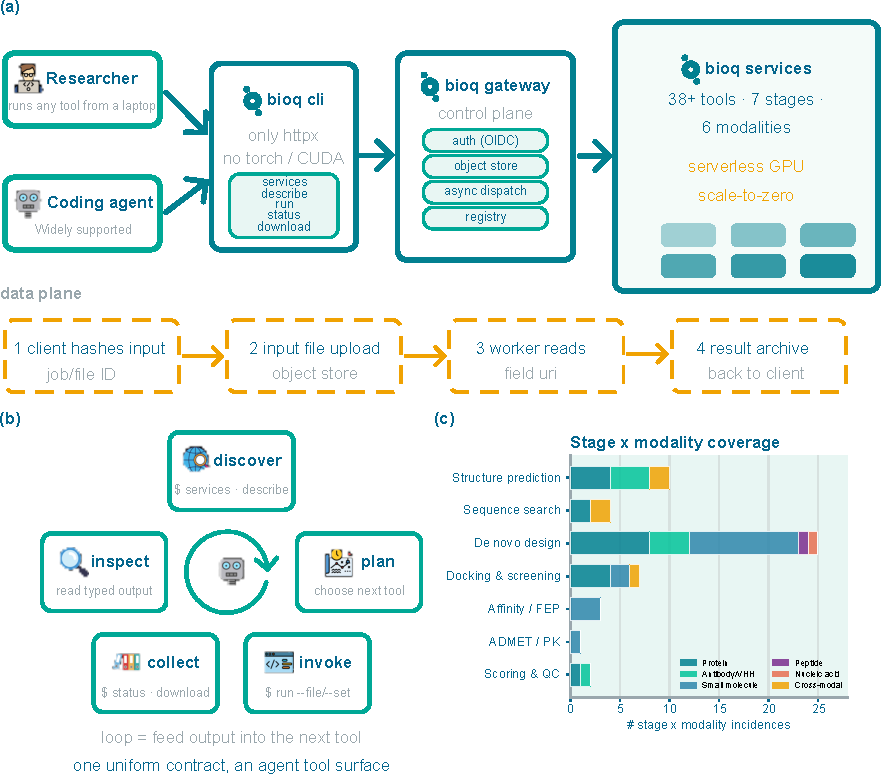
\includegraphics[width=\textwidth]{fig1_architecture}
\caption{\texttt{bioq} unifies a three-tier service architecture behind a
  common interface for researchers and coding agents. (a) The thin
  \texttt{bioq} client communicates with a control-plane gateway,
  which dispatches jobs to more than 38 serverless GPU and CPU
  services. Large inputs are transferred through content-addressed
  storage and bypass the request path. (b) Coding agents use the same
  \texttt{describe}/\texttt{run} contract to form a closed loop of
  tool discovery, invocation, result collection, inspection, and
  chaining. (c) Modality coverage by discovery stage,
  with one stacked horizontal bar per stage.}
\label{fig:architecture}
\end{figure*}

\subsection{A uniform, self-describing contract}\label{sec:contract}

Every tool, regardless of its native interface or input format, is
exposed through the same five subcommands: \texttt{bioq services}
lists the available services; \texttt{bioq describe <service>}
displays a service manifest; \texttt{bioq run <service> <endpoint>}
invokes an endpoint; and \texttt{bioq status} and \texttt{bioq
  download} retrieve job status and results, respectively. Each
manifest is machine-readable and specifies the endpoints exposed by
the service, the name and type of every parameter, and any required
file inputs.

Jobs are submitted using a uniform syntax:

\begin{verbatim}
bioq run <service> <endpoint> \
  --file field=path --set k=v --wait -o out
\end{verbatim}

The option \texttt{--output json} returns structured, machine-readable
output containing the job identifier and status. The manifest serves
both as human-readable documentation and as a schema from which an
agent can construct a valid invocation. Consequently, users and agents
need to learn only one interface to access the entire service fleet.

To assess fleet-wide adherence to this contract, we performed a
manifest-only audit of 30 deployed services comprising 141 endpoints,
including 68 asynchronous task endpoints invocable through
\texttt{bioq run}. Of these task endpoints, 98.5\,\% were fully
conformant, and the median per-service conformity score was 1.0,
demonstrating that the contract is implemented consistently across the
fleet (Figure S1).

\subsection{Data plane and dual-mode execution}\label{sec:dataplane}


To transfer the large files consumed and produced by these models,
\texttt{bioq} uses a content-addressed data plane. The client computes the
SHA-256 hash of each input, obtains a presigned object-storage URL
from the gateway, and uploads the file directly to object
storage. Large inputs, such as protein structures (PDB files) and
multiple-sequence-alignment (MSA) files, therefore bypass the
gateway's request path. Objects are deduplicated by content hash, so
an input already present in storage need not be uploaded again. The
gateway then passes the corresponding object URI to the job as
\texttt{field\_uri}, and the resulting artifacts are returned as a
single archive.

Each service image supports two execution modes: an asynchronous HTTP
job runner for cloud and serverless deployment, and a one-shot CLI
batch program invoked as \texttt{python -m server <endpoint>}. The same
image and parameter schema can therefore be used across managed
serverless platforms, self-managed clusters, HPC batch systems, and
local compute nodes, enabling reproducible execution without separate
deployment-specific implementations.

In the serverless mode, the gateway dispatches jobs to scale-to-zero
GPU functions \citep{jonas_cloud_2019}. When deployed on Alibaba Cloud
Function Compute (FC), worker instances are provisioned on demand,
billed according to job resource usage, and released when idle. This
model gives users access to GPU capacity without requiring them to
purchase, provision, or pay for idle hardware.


\subsection{Access modes}\label{sec:accessmodes}

\texttt{bioq} exposes the same contract to all consumers, whether human or
agent. Human users interact with it through the command line or shell
scripts. Autonomous coding agents use the identical interface, with
only a single client dependency to install: \texttt{services} and
\texttt{describe} provide structured tool discovery; \texttt{run},
together with \texttt{--file}, \texttt{--set}, and \texttt{--output
  json}, provides programmatic invocation; and a submit $\rightarrow$
poll $\rightarrow$ download $\rightarrow$ inspect loop enables the
output of one tool to be passed to the next
(Figure~\ref{fig:architecture}b). Because the interface is uniform,
self-describing, and machine-readable, agents can discover tools and
compose multistep workflows without requiring a bespoke adapter for
each service.


%% ---------------------------------------------------------------------------
%% 3. The service fleet
%% ---------------------------------------------------------------------------
\section{The service fleet}\label{sec:fleet}


The current fleet comprises 38 services spanning seven stages of the
discovery pipeline and six molecular modalities: proteins,
antibodies/VHHs, small molecules, peptides, nucleic acids, and
cross-modal systems (Figure~\ref{fig:architecture}c). Of these
services, 30 are currently deployed on our private serverless
infrastructure hosted on FC; these services constitute the set audited
in \S\ref{sec:contract}.

The fleet covers a broad range of computational tasks. It includes
AlphaFold, Boltz2, and ESMFold2 for protein structure prediction;
MMseqs2 \citep{steinegger_mmseqs2_2017} for sequence search;
RFdiffusion, ProteinMPNN, Genie3, and RFantibody for de novo design,
with RFantibody using an internal RoseTTAFold-2 (RF2) model for
structure prediction and scoring \citep{bennett_atomically_2026};
DiffDock, HADDOCK3 \citep{giulini_haddock3_2025}, and LightDock for
molecular docking; BindFlow and QligFEP for affinity and free-energy
estimation; OpenADMET \citep{fraser_mapping_2026} for ADMET
prediction; and DockQ \citep{basu_dockq_2016} and DeepRank-Ab
\citep{xu_deeprank-ab_2025} for model scoring. The full service list
and its per-tool citations are in Supplementary Table~S1.

The fleet is extensible by design. Adding a tool requires only a
container image that implements the shared service contract and a
corresponding registry entry. No modification to the client is
required, and the newly deployed tool becomes discoverable through
\texttt{bioq services}. The same architecture also allows the fleet to
track upstream development efficiently. Since each tool is isolated in
its own container and described declaratively, incorporating a new
upstream release (or an entirely new method) requires rebuilding only
the affected image, without altering any other service. The numbers
reported above therefore represent a snapshot of a fleet designed to
grow and evolve alongside the field.

%% ---------------------------------------------------------------------------
%% 4. Results
%% ---------------------------------------------------------------------------
\section{Results}\label{sec:results}

Because \texttt{bioq} addresses accessibility and integration rather
than model accuracy, we evaluate the platform's coverage and
operational characteristics without re-benchmarking the predictive
performance of the underlying models, which has been established in
their respective upstream studies. We organize the results around
three practical questions: how fragmented the underlying computational
ecosystem is; how effectively \texttt{bioq} shields end users from
this fragmentation; and how bioq-enabled workflows perform in terms of
scalability, cost, and real-world usability.


\subsection{Access barriers}\label{sec:access}

The diversity of the underlying software stacks makes it impractical
to consolidate the fleet into a single environment. An audit of all 38
services identified 15 distinct PyTorch versions, ranging from 1.12 to
2.12, across CUDA 11 and 12 and Python 3.9--3.12. In combination,
these dependencies form 23 distinct stack signatures. Among the 32
tools for which parseable upstream dependency specifications were
available, pairwise comparison showed that only 9.9\,\% of tool pairs
(49 of 496) were fully compatible, 48.6\,\% of tool pairs (241 of 496)
were hard-incompatible: their declared version constraints were
disjoint, so no shared environment could satisfy both
(Figure~S2). \texttt{bioq} hides this complexity behind a single
$\sim$1.8\,MB client whose only runtime dependency is \texttt{httpx}.

Hardware availability presents a separate barrier. Most services in
the fleet cannot run on the hardware available in a typical
researcher's laptop. An audit of per-service hardware requirements
showed that the GPU services generally require more memory than
laptop-class devices can provide. Among the 26 GPU services with
quantified minimum VRAM requirements, 24 require more than 4\,GB and
14 require more than 8\,GB (Figure~S3). \texttt{bioq} therefore
executes these services on remote, serverless GPUs rather than on the
client device.


\subsection{Scale and operating cost}\label{sec:scale}

For embarrassingly parallel screening and design workloads, serverless
dispatch provides throughput beyond that of a single workstation
without requiring users to orchestrate workers themselves. In batches
of 50 independent jobs, the observed speedup relative to serial
execution reached approximately 16.8$\times$ for PLIP,
10.6$\times$ for ProteinMPNN, and 10.4$\times$ for REINVENT, with
peak concurrency reaching approximately 49 worker instances across the
evaluated workloads (Figures~S4 and S5).

Because worker instances scale to zero when idle, compute costs are
incurred primarily during job execution rather than through continuous
GPU provisioning. Based on the public serverless pricing schedule, our
cost model estimates a weighted mean cost of approximately \$0.18 per
job and a duty-cycle break-even point of approximately 8.8\,\%
relative to an owned A100 GPU (Figure~S6). Serverless execution is
therefore economically favorable under the assumptions of this model
for bursty workloads that would otherwise leave dedicated hardware
idle for most of its lifetime.

Scaling on Function Compute (FC) is ultimately constrained by
cold-start latency and platform concurrency quotas. These limits affect
short jobs and large bursts in particular, although concurrency quotas
can be adjusted when additional capacity is required.


\subsection{Use case: a de novo antibody-design campaign}\label{sec:campaign}


As an end-to-end demonstration, we executed the RFantibody de novo
antibody-design pipeline entirely through \texttt{bioq}. The pipeline
comprises RFdiffusion for backbone generation, ProteinMPNN for
sequence design, and RoseTTAFold-2 (RF2) for structure prediction and
interface scoring \citep{bennett_atomically_2026}. For each target,
the complete workflow was launched from a laptop using three uniform
\texttt{bioq run} commands, without a local GPU, model installation,
or CUDA environment:

\begin{lstlisting}[language=bash,basicstyle=\ttfamily\footnotesize,breaklines=true]
bioq run rfantibody rfdiffusion --file target=target.pdb --file framework=vhh.pdb \
  --set num_designs=1000 --set hotspots=... --wait -o s1
bioq run rfantibody proteinmpnn --file input_quiver=s1/1_rfdiffusion.qv \
  --set seqs_per_struct=8 --wait -o s1
bioq run rfantibody rf2 --file input_quiver=s1/2_proteinmpnn.qv --wait -o s1
\end{lstlisting}

Although each stage uses a different model, \texttt{bioq} exposes all
three through the same execution contract. Across nine targets---seven
VHHs and two scFvs---the campaign generated 1,000 candidate backbones
per target and eight sequences per backbone, for a total of 72,000
designed sequences. All jobs were dispatched to the scale-to-zero GPU
workers described in \S\ref{sec:scale}, with no local model code, GPU
provisioning, or CUDA configuration.

We evaluated the designs using the in silico filters defined in the
original RFantibody study: interface predicted aligned error
($\mathrm{pAE}<10$\,\AA) and design--model CDR root-mean-square
deviation (RMSD) below 2\,\AA, where the latter measures
self-consistency between the designed backbone and the RF2-predicted
structure. Under the best-of-eight criterion used by the upstream
method, per-target acceptance rates ranged from 2.4\,\% to 70.6\,\%,
consistent with the broad in silico acceptance funnel reported in the
original study. Table~S2 reports the complete per-target funnel and a
comparison with the published RFantibody results. Figure~S7 visualizes
the per-target funnel, while Figures~S8 and S9 show the corresponding
interface-pAE and CDR-RMSD distributions.

The same execution pattern can be extended across independently
packaged services---for example, using RFdiffusion for backbone
generation, Boltz for structure prediction, and DockQ for
scoring---without changing the underlying contract. Importantly, the
acceptance rates reported here are computational filtering rates, not
experimental binding success rates. In the upstream study, the
experimental hit rate was at most 2\,\%, substantially lower than the
in silico acceptance rate \citep{bennett_atomically_2026}.

%% ---------------------------------------------------------------------------
%% 5. Discussion
%% ---------------------------------------------------------------------------
\section{Discussion}\label{sec:discussion}

\texttt{bioq} shifts access to computational models from tool-specific
local installations to a uniform, remotely executable service
contract. This approach removes much of the software-compatibility and
hardware-provisioning burden for users who need to combine multiple
tools, but it also introduces several trade-offs. Serverless
throughput is bounded by cold-start latency and platform concurrency
limits, and its economic advantage depends strongly on workload duty
cycle. Above the estimated break-even point, dedicated GPU
infrastructure is likely to be more cost-effective than cloud platform
serverless computation.

The service fleet is curated and centrally versioned. This design makes
it possible to add new methods and track upstream releases by rebuilding
individual containers without disrupting the remainder of the fleet.
For users who depend on multiple tools, such isolation avoids the
``incompatibility tax'' associated with maintaining mutually conflicting
software environments. However, formal policies for release versioning,
deprecation, backward compatibility, and long-term reproducibility
remain to be established.

The current data plane assumes access to cloud-compatible object
storage. Although this dependency can be mitigated through self-hosted
storage and the CLI batch mode for HPC environments, fully disconnected
or tightly regulated deployments may require additional integration.
Workflow chaining is also currently implemented through client-side
scripts. A declarative workflow layer, including explicit provenance,
caching, retries, and dependency management, is left for future work;
the uniform, self-describing contract introduced here provides the
foundation on which such a layer can be built.


%% ---------------------------------------------------------------------------
%% Acknowledgments
%% ---------------------------------------------------------------------------
\section*{Acknowledgments}\label{sec:acknowledgments}

The authors thank the developers and maintainers of the open-source
methods and platforms underlying this work for releasing their code
and model weights, including AlphaFold, RoseTTAFold-2, ColabFold,
RFdiffusion, ProteinMPNN, RFantibody, and MMseqs2, among others. LLM
tools were used to assist with coding and language polishing. All
scientific claims, analyses, and generated text were reviewed and
verified by the authors, who take full responsibility for the final
manuscript.

% Supplementary figures (S1--S8) and tables (S1, S2) are compiled as a separate
% PDF: see supplementary.tex (built by build.sh in the same pass).

%% ---------------------------------------------------------------------------
%% Bibliography
%% ---------------------------------------------------------------------------
% Author--year citations (matches the OUP/Bioinformatics author--date CSL used for
% the Word render). For numbered citations, switch to `numbered` in the class
% options and use \bibliographystyle{oup-plain} below. oup-abbrvnat-et-al truncates
% long author lists in the reference list to 6 authors + "et al." (edit the .bst).
\bibliographystyle{oup-abbrvnat-et-al}
\bibliography{references-escaped}

\end{document}
